\documentclass[12pt,a4paper,openright,twoside]{book}
\usepackage[utf8]{inputenc}
\usepackage[italian]{babel}  
\usepackage{disi-thesis}
\usepackage{code-lstlistings}
\usepackage{notes}
\usepackage{shortcuts}
\usepackage{acronym}

\school{\unibo}
\programme{Corso di Laurea in Ingegneria e Scienze Informatiche}
\title{Sviluppo di un pannello Web a supporto di un filtro DNS}
\author{Alessandro Valmori}
\date{\today}
\subject{Programmazione ad Oggetti}
\supervisor{Prof. Mirko Viroli}
\cosupervisor{Dott. Nicolas Farabegoli}
\session{II}
\academicyear{2024-2025}


\mainlinespacing{1.241} % line spacing in mainmatter, comment to default (1)

\begin{document}

\frontmatter\frontispiece

\begin{abstract}
    Nel contesto aziendale moderno, la necessità di analizzare e monitorare il traffico internet filtrato è diventata sempre più critica per garantire sicurezza e conformità. Le aziende richiedono strumenti di visualizzazione che permettano di esaminare i dati di filtraggio DNS senza rischi di modifiche accidentali alle configurazioni di sicurezza. In questo scenario, l'implementazione di sistemi di autenticazione robusti e sicuri rappresenta un elemento fondamentale per proteggere dati sensibili e garantire accesso controllato alle informazioni aziendali.

    Questa tesi descrive lo sviluppo di una dashboard web in modalità readonly per la visualizzazione e l'analisi dei dati di filtraggio DNS, realizzata in collaborazione con FlashStart SRL, azienda leader nel settore del filtraggio dei contenuti web. Il progetto nasce come soluzione temporanea per colmare una lacuna funzionale della piattaforma esistente, fornendo ai clienti dell'azienda uno strumento dedicato all'analisi dei dati fino al rilascio della nuova infrastruttura aziendale.

    L'obiettivo del lavoro è duplice: sviluppare un'applicazione web funzionale e sicura che implementi meccanismi di autenticazione avanzati per proteggere l'accesso ai dati sensibili, e analizzare criticamente come i principi della programmazione orientata agli oggetti guidino le scelte architetturali in un contesto industriale reale. Il sistema implementa un'architettura full-stack moderna, utilizzando tecnologie reattive per garantire scalabilità ed efficienza, con particolare attenzione alla sicurezza attraverso sistemi di autenticazione stateless e gestione sicura delle sessioni utente.

    Questo lavoro rappresenta un esempio concreto di come i principi teorici dell'ingegneria del software trovino applicazione pratica nella risoluzione di problemi aziendali, evidenziando l'importanza dei design pattern e delle metodologie orientate agli oggetti nello sviluppo di software industriale.

\end{abstract}

\begin{dedication} % this is optional
    Alla mia famiglia, a Saul detto el Butre, a Linda e ai miei amici.
\end{dedication}

%----------------------------------------------------------------------------------------
\tableofcontents
%\listoffigures     % (optional) comment if empty
%\lstlistoflistings % (optional) comment if empty
%----------------------------------------------------------------------------------------

\mainmatter

%----------------------------------------------------------------------------------------
\chapter{Introduzione}
\label{chap:introduzione}

\section{Contesto Aziendale e Motivazione del Progetto}
\label{sec:contesto_e_motivazione}

Il presente lavoro di tesi si inserisce in un contesto industriale specifico, frutto della collaborazione con FlashStart SRL, un'azienda italiana con sede a Cesena, specializzata nello sviluppo e nella fornitura di soluzioni di filtraggio dei contenuti e protezione da minacce informatiche basate su tecnologia DNS (Domain Name System). I servizi offerti da FlashStart si rivolgono a una clientela diversificata, che include aziende, istituzioni educative e pubbliche amministrazioni, fornendo loro strumenti per garantire una navigazione sicura e controllata.

Al momento dell'inizio del percorso di tirocinio, nel mese di giugno 2025, l'azienda si trovava in una fase di significativa evoluzione tecnologica e strategica. Era infatti in corso un processo di completa reingegnerizzazione della propria piattaforma di gestione, la dashboard utilizzata dai clienti per configurare e monitorare il servizio di filtraggio. Questo processo, unito a un'operazione di rebranding aziendale, mirava a modernizzare l'infrastruttura e l'esperienza utente, con un rilascio previsto per novembre 2025.

In questo scenario di transizione, è emersa una criticità tanto specifica quanto urgente. La piattaforma allora in uso, pur essendo efficace per la gestione delle policy di protezione, presentava una notevole lacuna funzionale: l'assenza di una modalità di consultazione dei dati in sola lettura (readonly). Gli utenti, in particolare gli amministratori di rete e i responsabili IT, manifestavano la crescente necessità di poter analizzare i report e le statistiche di navigazione senza avere i permessi di modifica, per evitare alterazioni accidentali delle configurazioni di sicurezza.

Il progetto di tesi nasce per rispondere a questa precisa esigenza. Data l'impossibilità di attendere il rilascio della nuova piattaforma, si è optato per lo sviluppo di una soluzione tattica e mirata: un'applicazione web temporanea, concepita come "ponte" (bridge) tecnologico. Lo scopo primario di questa applicazione è fornire ai clienti un pannello di controllo readonly per le funzionalità standard di analisi dei dati, garantendo continuità operativa e soddisfacendo le richieste del mercato fino alla migrazione sulla nuova infrastruttura. Questo lavoro di tesi documenta pertanto non solo la realizzazione di un prodotto software, ma anche l'approccio ingegneristico adottato per sviluppare una soluzione efficace e affidabile in un contesto agile e con vincoli temporali definiti.

\section{Obiettivi della Tesi}
\label{sec:obiettivi_tesi}

A partire dal contesto delineato, questo elaborato si pone obiettivi che trascendono la semplice descrizione di un prodotto software, per configurarsi come un'analisi approfondita delle metodologie di ingegneria del software applicate a un caso di studio reale. Il fine principale della tesi è, pertanto, analizzare e documentare come i paradigmi della Programmazione Orientata agli Oggetti (OOP) e le relative pratiche di progettazione, quali i design pattern, vengano impiegati per realizzare un'applicazione web complessa in un contesto industriale. Si intende dimostrare come tali principi, spesso affrontati in ambito teorico, rappresentino strumenti pratici e fondamentali per guidare le scelte architetturali e per garantire qualità essenziali come la manutenibilità, la scalabilità e la robustezza del software, specialmente quando si opera con vincoli di tempo e risorse.

Per supportare tale analisi, un primo passo fondamentale sarà la documentazione completa e dettagliata dell'architettura full-stack dell'applicazione. Verrà illustrato il flusso di dati e le interazioni tra il frontend, sviluppato in React con TypeScript, e il backend, basato su un modello di programmazione reattiva in Java. Questo esame non si limiterà a una descrizione statica, ma includerà un'analisi critica delle decisioni tecniche prese durante lo sviluppo, giustificando la scelta dello stack tecnologico e approfondendo l'implementazione di componenti chiave come il sistema di autenticazione sicuro basato su token JWT e l'integrazione con le API esterne di FlashStart.

Il cuore analitico della tesi si concentrerà sull'applicazione pratica dei Design Pattern. Verranno identificati e discussi esempi concreti di pattern implementati nel codice sorgente, spiegando per ciascuno il problema che risolve e i benefici apportati in termini di flessibilità e organizzazione del codice. In questo modo, si intende creare un collegamento esplicito tra i concetti teorici dell'ingegneria del software e la loro implementazione pratica. Particolare attenzione sarà data a come le scelte di design abbiano promosso un'architettura dinamica e facilmente manutenibile; un requisito fondamentale dato che l'applicazione doveva interfacciarsi con servizi interni di FlashStart a loro volta in piena fase di reingegnerizzazione. Verrà quindi evidenziato come le decisioni di design non siano state casuali, ma guidate da principi consolidati volti a massimizzare l'efficienza e la qualità, nel pieno rispetto della natura strategica ma temporanea del progetto.


\section{Panoramica dello Stack Tecnologico}
\label{sec:stack_tecnologico}

La realizzazione di un'applicazione robusta, scalabile e sicura, pur in un contesto di sviluppo agile e a breve termine, ha richiesto un'attenta selezione delle tecnologie costitutive. L'architettura del sistema è stata progettata per essere moderna e reattiva, garantendo un'esperienza utente fluida e un uso efficiente delle risorse server. Ogni componente dello stack, dal backend al frontend, fino all'infrastruttura di deployment, è stato scelto per rispondere a precise esigenze di progetto.

Il cuore pulsante dell'applicazione risiede nel backend, sviluppato in Java 17 e fondato sul framework Spring Boot. Per questo progetto è stato adottato un paradigma di programmazione completamente reattivo, utilizzando Spring WebFlux anziché il tradizionale Spring MVC. Questa scelta strategica si basa sulla natura dell'applicazione, intrinsecamente legata a operazioni di I/O (input/output) come le chiamate verso API esterne e l'accesso al database. Il modello non bloccante di WebFlux permette di gestire un elevato numero di connessioni concorrenti con un numero limitato di thread, ottimizzando le risorse e garantendo bassa latenza. Inoltre, il backend assume un ruolo centrale di API Gateway grazie all'integrazione con Spring Cloud Gateway. Questa componente orchestra il traffico di rete, indirizzando le richieste del client verso le API interne dell'applicazione o fungendo da proxy sicuro verso i due distinti endpoint di FlashStart, applicando filtri personalizzati per l'autenticazione e l'arricchimento delle chiamate.

Per l'interfaccia utente è stata realizzata una Single Page Application (SPA) utilizzando React, una delle librerie JavaScript più diffuse per la creazione di interfacce complesse e performanti. L'adozione di TypeScript ha introdotto la tipizzazione statica nel codice frontend, un elemento cruciale per aumentare la robustezza, la manutenibilità e la chiarezza del codice, riducendo la probabilità di errori a runtime. La comunicazione asincrona con il backend avviene tramite chiamate HTTP gestite dalla libreria axios, configurata con intercettori specifici per aggiungere automaticamente i token di autenticazione alle richieste e per gestire in modo trasparente la logica di rinnovo dei token in caso di sessione scaduta, come definito in axiosInstance.ts.

La persistenza dei dati, limitata alle informazioni su utenti e token per la gestione delle sessioni, è affidata a PostgreSQL, un database relazionale open-source rinomato per la sua stabilità e le sue funzionalità avanzate. Per mantenere la coerenza con l'approccio reattivo del backend, l'accesso al database è gestito tramite Spring Data R2DBC (Reactive Relational Database Connectivity). Questo permette di estendere il paradigma non bloccante fino al livello di accesso ai dati, evitando colli di bottiglia e garantendo che l'intera catena di elaborazione di una richiesta, dalla ricezione alla risposta, rimanga asincrona.

La sicurezza dell'applicazione è un pilastro fondamentale dell'architettura. Il sistema di autenticazione è stateless e si basa su JSON Web Tokens (JWT), che vengono trasmessi dal client nell'header di ogni richiesta autorizzativa. Per mitigare i rischi legati a token di lunga durata, è stato implementato un meccanismo di sicurezza avanzato noto come rotazione dei refresh token. Come visibile nel AuthenticationService, ogni volta che un refresh token viene utilizzato con successo per ottenere un nuovo access token, esso viene immediatamente invalidato e sostituito da uno nuovo. Questa strategia riduce drasticamente la finestra temporale in cui un token compromesso potrebbe essere sfruttato, aumentando significativamente la sicurezza complessiva delle sessioni utente.

Infine, l'intera infrastruttura è gestita tramite un approccio DevOps moderno. L'applicazione è interamente containerizzata utilizzando Docker, e la sua architettura multi-servizio (backend, frontend web server e database) è definita tramite file docker-compose.yaml. Questo garantisce la portabilità e la riproducibilità dell'ambiente su macchine diverse. Il ciclo di vita dello sviluppo è automatizzato da una pipeline di Continuous Integration e Continuous Deployment (CI/CD) ibrida, che si avvale di GitHub Actions per l'orchestrazione dei flussi di lavoro e di un runner self-hosted, installato direttamente sul server di destinazione, per eseguire in modo sicuro le operazioni di build e deployment.

%----------------------------------------------------------------------------------------
\chapter{Background}
\label{chap:background}

% Introduzione al capitolo
Il presente capitolo si prefigge di delineare il contesto teorico e tecnologico che funge da fondamento per lo sviluppo del pannello web oggetto di questa tesi.  Per giustificare le decisioni architetturali e tecnologiche adottate, verranno esplorate le aree di ricerca che hanno guidato le scelte progettuali e implementative.  L'analisi spazierà dai fondamenti della Programmazione Orientata agli Oggetti (OOP) e dei design pattern, fino alle architetture reattive e alle metodologie DevOps, per concludere con uno sguardo allo stato dell'arte dei sistemi di filtraggio DNS in cui il progetto si inserisce.

\section{Architetture Reattive e Programmazione Non-bloccante}
\label{sec:architetture_reattive}

Le architetture reattive sono diventate fondamentali per costruire applicazioni web capaci di gestire alta concorrenza e grandi volumi di dati mantenendo responsività. La programmazione reattiva è un paradigma focalizzato sui flussi di dati (data streams) e sulla propagazione del cambiamento; le applicazioni "reagiscono" ai dati man mano che diventano disponibili. I suoi benefici principali sono una migliore responsività (le operazioni non bloccanti evitano che l'applicazione si fermi in attesa di I/O), resilienza (gestione degli errori integrata nei flussi), elasticità e un uso efficiente delle risorse.

Spring WebFlux è il modulo di Spring che permette di creare applicazioni web reattive in Java. È costruito su Project Reactor, che fornisce i tipi \texttt{Mono<T>} (per 0 o 1 elemento) e \texttt{Flux<T>} (per 0 o N elementi). Le sue caratteristiche chiave sono l'I/O non bloccante, che permette di servire molte connessioni con pochi thread, il supporto alla "backpressure" per evitare sovraccarichi, e la possibilità di comporre logica asincrona in modo dichiarativo.

Un aspetto interessante è la distinzione tra Object-Oriented Reactive Programming (OORP), dove si usano oggetti per comporre flussi reattivi, e Reactive Object-Oriented Programming (ROOP), dove gli oggetti stessi sono flussi di stato reattivo \cite{Boix2013OORP}. Spring WebFlux tende a favorire un approccio OORP, dove i servizi e i controller orchestrano e manipolano i flussi \texttt{Flux} e \texttt{Mono}.

\section{Pattern Architetturali per Sistemi Reattivi}
\label{sec:pattern_reattivi}

L'adozione di un'architettura reattiva, sebbene potente, introduce sfide di progettazione che richiedono soluzioni più evolute rispetto ai classici design pattern. Il tradizionale pattern Observer, pur essendo fondamentale, può infatti mostrare limiti in contesti complessi, come la potenziale incapacità di aggiornare correttamente gli oggetti, l'esecuzione di aggiornamenti ridondanti o in ordine errato (causando "glitch") e la creazione di dipendenze circolari. Per superare queste criticità, sono emersi pattern più sofisticati come il pattern REACTOR \cite{Mijac2021Reactor}. Questo pattern utilizza un grafo di dipendenze per gestire le reazioni a catena, assicurando che gli aggiornamenti avvengano in modo ordinato e consistente tramite ordinamento topologico. È pensato per scenari in cui il cambiamento di stato di un oggetto richiede una reazione automatica in tutti gli oggetti dipendenti, situazione comune in interfacce grafiche, fogli di calcolo e animazioni. Sebbene la sua implementazione di riferimento sia in C\#, i concetti sono perfettamente applicabili al contesto Java di questo progetto.

A livello di interfaccia utente, il pattern DCRC (Dynamically Coalescing Reactive Chains) \cite{Oliveira2024DCRC} affronta problemi simili, riducendo i "glitch" visivi nelle GUI web raggruppando catene di eventi per garantire aggiornamenti ordinati. La progressione da Observer a pattern come REACTOR (per il backend) e DCRC (per il frontend) evidenzia una maturazione nel modo in cui le applicazioni moderne gestiscono cambiamenti di stato complessi, un tema centrale per questo lavoro di tesi che integra OOP e programmazione reattiva.

\section{Sicurezza nelle Applicazioni Web}
\label{sec:sicurezza_web}

La sicurezza è un aspetto non negoziabile, specialmente in un'applicazione che gestisce il monitoraggio di un filtro DNS. Il meccanismo di autenticazione scelto per questo progetto è basato su JSON Web Tokens (JWT), uno standard aperto per creare token di accesso che contengono "claim" (asserzioni) su un utente. Un JWT è composto da un Header, un Payload e una Signature, che ne garantisce l'integrità e l'autenticità.

Seguendo le best practice di sicurezza, l'architettura adotta token di accesso a breve scadenza (access token) e token di aggiornamento a lunga scadenza (refresh token). Una misura di sicurezza cruciale implementata è la rotazione dei refresh token: quando un refresh token viene usato, viene invalidato e sostituito con uno nuovo. Questa tecnica aiuta a rilevare eventuali furti e limita drasticamente i danni in caso di compromissione del token. Questo approccio, sebbene aumenti la sicurezza, introduce un leggero grado di "statefulness" in un sistema altrimenti stateless, poiché il server deve mantenere traccia dei token validi, un compromesso progettuale importante discusso in questa tesi.

\section{Metodologie DevOps e Containerizzazione}
\label{sec:devops}

Le pratiche DevOps e la containerizzazione sono standard moderni per aumentare l'efficienza e l'affidabilità del ciclo di vita del software. Per questo progetto è stato utilizzato Docker, una piattaforma che automatizza il deployment di applicazioni all'interno di container software. I container incapsulano l'applicazione e tutte le sue dipendenze, garantendo che funzioni in modo coerente in qualsiasi ambiente ed eliminando il classico problema del "funziona sulla mia macchina". I benefici includono consistenza, isolamento, gestione semplificata delle dipendenze e scalabilità.

Il ciclo di vita del software è automatizzato tramite una pipeline di Continuous Integration/Continuous Deployment (CI/CD). Questo progetto sfrutta una soluzione ibrida con GitHub Actions per l'orchestrazione e runner self-hosted per l'esecuzione dei job di deployment. Questo approccio combina la comodità della definizione delle pipeline su GitHub con la sicurezza e la flessibilità di eseguire il deployment su macchine controllate direttamente dall'azienda.

\section{Stato dell'Arte: Sistemi di Filtraggio DNS}
\label{sec:dns_filtering}

Per comprendere appieno il contesto applicativo, è essenziale analizzare lo stato dell'arte del filtraggio DNS. Il Domain Name System (DNS) è il sistema che traduce i nomi di dominio (es. www.google.com) in indirizzi IP. Il filtraggio DNS sfrutta questo meccanismo per bloccare l'accesso a domini malevoli o indesiderati, intercettando le richieste e rispondendo con l'indirizzo di una pagina di blocco o facendo fallire la risoluzione. Le moderne soluzioni di filtraggio, come quelle di FlashStart, utilizzano blacklist, whitelist e, sempre più, sistemi basati su Intelligenza Artificiale (AI) e Machine Learning (ML) per classificare dinamicamente i domini e proteggere dalle minacce zero-day.

Il pannello web sviluppato in questa tesi non è il filtro stesso, ma un'interfaccia di gestione e analisi per il sistema di filtraggio. Questo implica che la sua architettura deve essere progettata per interagire efficacemente con un'infrastruttura di sicurezza critica e ad alte prestazioni, presentando i dati in modo chiaro e supportando la configurazione delle policy che verranno poi applicate dai motori di filtraggio DNS.
%----------------------------------------------------------------------------------------
\chapter{Analisi}
\label{chap:analisi}

% Introduzione al capitolo
In questo capitolo si definiscono le fondamenta progettuali dell'applicazione web. Partendo dal contesto aziendale e dalle motivazioni esposte nell'Introduzione, verranno delineati in modo formale i requisiti che la soluzione software dovrà soddisfare. L'analisi si articola nella definizione delle funzionalità attese (requisiti funzionali), dei vincoli qualitativi e operativi (requisiti non funzionali) e del panorama di sistemi esterni con cui l'applicazione dovrà necessariamente interagire. Questo capitolo ha lo scopo di definire il perimetro e gli obiettivi del sistema, fungendo da guida per le successive fasi di progettazione e implementazione.

\section{Analisi dei Requisiti}
\label{sec:analisi_requisiti}
La definizione dei requisiti costituisce il primo passo del processo ingegneristico, traducendo le esigenze degli stakeholder in specifiche precise. Tali requisiti vengono classificati in funzionali, che descrivono il comportamento del sistema, e non funzionali, che ne specificano le proprietà e i vincoli.

\subsection{Requisiti Funzionali}
\label{subsec:req_funzionali}
I requisiti funzionali descrivono le capacità che l'applicazione dovrà offrire ai suoi utenti per risolvere il problema di business identificato. Il sistema dovrà quindi essere in grado di:

\begin{itemize}
    \item \textbf{RF1: Fornire un accesso autenticato.} Il sistema dovrà garantire che solo gli utenti autorizzati possano accedere ai dati. Sarà necessario un meccanismo di login basato su credenziali (e-mail e password) per proteggere l'accesso alle informazioni.

    \item \textbf{RF2: Presentare una dashboard di riepilogo.} Dopo l'autenticazione, l'applicazione dovrà visualizzare una pagina principale che offra una sintesi immediata dello stato del servizio, presentando statistiche aggregate sul traffico DNS e sulle minacce rilevate in un determinato intervallo temporale.

    \item \textbf{RF3: Permettere la consultazione delle policy di protezione.} L'utente dovrà poter navigare e ispezionare le configurazioni di protezione attive associate ai propri profili. Ciò include la visualizzazione delle categorie di contenuti filtrate, delle regole di geo-blocking e delle liste di eccezioni (blacklist e whitelist).

    \item \textbf{RF4: Mostrare le configurazioni di rete.} Sarà necessario fornire una sezione dedicata alla visualizzazione delle reti associate all'account del cliente, distinguendo tra indirizzi IP statici, utenze dinamiche e connessioni sicure tramite protocolli crittografati (DoH/DoT).

    \item \textbf{RF5: Offrire uno strumento di analisi per domini specifici.} L'applicazione dovrà includere una funzionalità di "lookup" che permetta all'utente di interrogare lo stato di un singolo dominio per verificare come verrebbe gestito dalle policy di ogni profilo (se bloccato o permesso) e per quale motivo.

    \item \textbf{RF6: Gestire il contesto multi-profilo e multi-cliente.} Poiché un utente può gestire più clienti e ciascun cliente può avere più profili di protezione, l'interfaccia dovrà permettere una facile selezione del contesto (cliente e profilo) per cui si desidera visualizzare i dati.
\end{itemize}

\subsection{Requisiti Non Funzionali}
\label{subsec:req_non_funzionali}
I requisiti non funzionali impongono vincoli sulla qualità e sulle modalità operative del sistema, influenzando profondamente le scelte architetturali.

\begin{itemize}
    \item \textbf{RNF1: Modalità di Sola Lettura.} Si tratta del requisito non funzionale più stringente: l'applicazione dovrà operare esclusivamente in modalità di consultazione. Nessuna funzionalità di modifica, creazione o cancellazione dei dati e delle configurazioni dovrà essere progettata o implementata.

    \item \textbf{RNF2: Alte Prestazioni e Reattività.} L'architettura dovrà essere progettata per essere performante ed efficiente, specialmente nella gestione delle operazioni di I/O verso i servizi esterni. Si predilige un modello di programmazione asincrono e non bloccante per il backend, al fine di garantire bassa latenza e un uso ottimale delle risorse computazionali.

    \item \textbf{RNF3: Sicurezza delle Sessioni Utente.} Il meccanismo di autenticazione dovrà essere di tipo stateless, per favorire la scalabilità, ma al contempo garantire un'elevata sicurezza. Per mitigare i rischi associati a token di lunga durata, si dovrà studiare e implementare una strategia di rotazione dei token, in particolare per i refresh token utilizzati per il rinnovo delle sessioni.

    \item \textbf{RNF4: Portabilità e Standardizzazione dell'Ambiente.} La soluzione software dovrà essere pacchettizzata in modo da garantire la coerenza e la riproducibilità dell'ambiente operativo. L'adozione della tecnologia di containerizzazione, come Docker, è identificata come la scelta strategica per raggiungere questo obiettivo.

    \item \textbf{RNF5: Vincoli di Progetto.} Lo sviluppo del sistema è vincolato da una precisa finestra temporale, essendo una soluzione "ponte" strategica. Questo requisito impone l'adozione di un approccio agile, favorendo scelte tecnologiche e architetturali che bilancino la velocità di realizzazione con la robustezza e la manutenibilità necessarie per un prodotto di livello industriale.
\end{itemize}

\section{Analisi del Contesto e delle Integrazioni}
\label{sec:analisi_contesto}
L'applicazione oggetto di studio non è un sistema autocontenuto, ma deve operare all'interno dell'ecosistema tecnologico di FlashStart per adempiere ai suoi requisiti funzionali. In particolare, per recuperare i dati necessari alla visualizzazione (come report, policy di protezione e configurazioni di rete), l'applicazione dovrà interfacciarsi con dei servizi API preesistenti.

Un'analisi dell'infrastruttura esistente ha identificato due distinti endpoint di servizio che espongono le informazioni richieste:
\begin{itemize}
    \item \textbf{Endpoint API HQ}: Un servizio specializzato che fornisce funzionalità di diagnostica e amministrazione. Ai fini di questo progetto, l'endpoint di maggior interesse è quello relativo al "lookup" di un dominio, che ne restituisce lo stato di filtraggio. Per comunicare con questo servizio, le richieste HTTP devono essere autenticate tramite il meccanismo di Basic Auth.

    \item \textbf{Endpoint API Principale (fsflt)}: Costituisce la fonte dati primaria per la maggior parte delle funzionalità del pannello. Da questo servizio è possibile recuperare tutte le informazioni operative, tra cui le configurazioni dei profili, le liste di protezione, i dati statistici per i report e l'elenco delle reti dei clienti. Le richieste a questo endpoint richiedono un'autenticazione basata su una chiave API (API key) univoca, associata all'utente che effettua la chiamata.
\end{itemize}
La necessità di interagire con questi due sistemi eterogenei, ciascuno con un proprio meccanismo di autenticazione, rappresenta un vincolo tecnico significativo. La soluzione software dovrà essere in grado di gestire questa complessità, orchestrando le chiamate verso entrambi gli endpoint per aggregare e presentare i dati all'utente in modo trasparente.
%----------------------------------------------------------------------------------------
\chapter{Design}
\label{chap:design}

% Introduzione al capitolo
Questo capitolo illustra la progettazione architetturale e di dettaglio dell'applicazione web, rispondendo ai requisiti funzionali e non funzionali definiti nel capitolo di Analisi. Verranno descritte le scelte strategiche relative alla struttura del software, le interazioni tra i componenti e i design pattern della programmazione orientata agli oggetti impiegati per garantire un'architettura robusta, manutenibile e scalabile.

\section{Progettazione dell'Architettura di Alto Livello}
\label{sec:design_architettura}

Per rispondere ai requisiti di portabilità e riproducibilità degli ambienti (RNF4), il sistema è stato progettato secondo un'architettura a servizi. Questo approccio favorisce una netta separazione delle responsabilità (Separation of Concerns), disaccoppiando i componenti logici principali, semplificandone lo sviluppo e garantendo la coerenza del sistema nelle diverse fasi del suo ciclo di vita.

La struttura logica del sistema è decomposta in tre componenti principali:

\begin{itemize}
    \item \textbf{Componente di Presentazione (Frontend)}: Questo componente ha la responsabilità di gestire l'interfaccia utente. È disegnato come una Single Page Application (SPA) servita da un web server. Il suo unico scopo è renderizzare le viste, gestire le interazioni con l'utente e comunicare con il componente applicativo per il recupero e la visualizzazione dei dati.

    \item \textbf{Componente Applicativo (Backend)}: Rappresenta il nucleo logico del sistema e agisce come unico punto di contatto per il componente di presentazione. Il suo design prevede una duplice responsabilità:
          \begin{enumerate}
              \item Gestire la logica di business interna, come l'autenticazione degli utenti e la gestione delle sessioni.
              \item Fungere da intermediario (secondo il pattern Architetturale API Gateway) verso i servizi esterni, astraendo la loro complessità dal frontend.
          \end{enumerate}

    \item \textbf{Componente di Persistenza Dati (Database)}: Questo componente è dedicato alla memorizzazione e al recupero dei dati necessari al funzionamento intrinseco dell'applicazione. In accordo con il requisito di sola lettura (RNF1) per i dati di business, il suo perimetro è strettamente limitato alla persistenza dei dati di sessione e delle anagrafiche utente.
\end{itemize}

Il flusso di interazione tra questi componenti è lineare e disaccoppiato. Il client utente interagisce esclusivamente con il Componente di Presentazione. Le richieste di dati vengono inoltrate da quest'ultimo al Componente Applicativo, che si occupa di elaborarle, interagendo a sua volta con il Componente di Persistenza per le operazioni relative all'autenticazione, o con i sistemi esterni (come descritto in Sezione \ref{sec:analisi_contesto}) per i dati di business.

\vspace{1cm} % Spazio per il diagramma

\begin{figure}[h!]
    \centering
    % \includegraphics[width=\textwidth]{path/to/your/logical-architecture-diagram.png}
    \fbox{Spazio per il diagramma dell'architettura logica (Componenti)}
    \caption{Diagramma dell'architettura logica di sistema, che illustra i componenti principali e i loro flussi di interazione.}
    \label{fig:logical_architecture_diagram}
\end{figure}

\vspace{1cm} % Spazio dopo il diagramma

Questa architettura a tre livelli logici permette di isolare le diverse responsabilità, migliorando la coesione di ciascun componente e riducendo l'accoppiamento tra di essi, a totale beneficio della manutenibilità e della testabilità del sistema.
\section{Design del Backend e Pattern OOP Applicati}
\label{sec:design_backend_oop}

Il componente backend rappresenta il nucleo logico dell'intera applicazione. La sua progettazione è stata affrontata con un approccio orientato agli oggetti, con l'obiettivo di creare un sistema modulare, poco accoppiato e facilmente estensibile. Per raggiungere tale scopo, sono stati impiegati diversi design pattern fondamentali, scelti per risolvere specifiche problematiche emerse durante la fase di analisi.

\subsection{Pattern Factory Method per la Creazione di Filtri Gateway}
\label{subsec:design_factory}

\paragraph{Problema di Design}
Dall'analisi delle integrazioni (Sezione \ref{sec:analisi_contesto}) è emersa la necessità di arricchire le richieste inoltrate ai due diversi endpoint esterni (API HQ e API Principale) con meccanismi di autenticazione differenti (Basic Auth per uno, API Key per l'altro). La sfida di design consisteva nel trovare un modo flessibile ed estensibile per creare e applicare queste logiche di modifica delle richieste in modo dinamico e disaccoppiato dalla configurazione delle rotte.

\paragraph{Soluzione di Design}
Per risolvere questo problema, è stato adottato il pattern creazionale \textbf{Factory Method}. Il design prevede la definizione di una interfaccia o classe base astratta, la \texttt{GatewayFilterFactory}, che dichiara un "metodo fabbrica" (\textit{factory method}) per la creazione di oggetti di tipo \texttt{GatewayFilter}. Un \texttt{GatewayFilter} è un oggetto la cui responsabilità è intercettare e modificare una richiesta HTTP.

Il design si completa con la creazione di due classi "fabbrica" concrete:
\begin{itemize}
    \item \texttt{ApiHqAuthGatewayFilterFactory}: Una fabbrica concreta che implementa il factory method per produrre un'istanza di \texttt{GatewayFilter} specializzata nell'aggiungere l'header di autenticazione Basic Auth, necessario per le chiamate verso l'endpoint API HQ.
    \item \texttt{FsfltApiKeyGatewayFilterFactory}: Un'altra fabbrica concreta il cui factory method produce un'istanza di \texttt{GatewayFilter} che si occupa di recuperare la chiave API dell'utente autenticato e di inserirla in un header specifico per le chiamate verso l'API Principale.
\end{itemize}
Questo approccio delega la responsabilità dell'istanziazione dei filtri alle sottoclassi, permettendo al sistema principale di configurazione delle rotte di operare a un alto livello di astrazione, senza conoscere i dettagli concreti di ciascun filtro. Ciò aumenta la modularità e semplifica l'eventuale aggiunta di nuovi filtri in futuro.

\vspace{1cm}
\begin{figure}[h!]
    \centering
    % \includegraphics[width=0.8\textwidth]{path/to/your/factory-method-uml.png}
    \fbox{Spazio per il diagramma delle classi UML del pattern Factory Method}
    \caption{Diagramma delle classi che illustra l'applicazione del pattern Factory Method per la creazione dei filtri del gateway.}
    \label{fig:factory_method_uml}
\end{figure}
\vspace{1cm}

\subsection{Pattern Singleton per la Gestione dei Servizi}
\label{subsec:design_singleton}

\paragraph{Problema di Design}
Molti componenti del backend, come i servizi per la gestione della logica di business (es. autenticazione, generazione JWT) o i repository per l'accesso ai dati, sono intrinsecamente \textit{stateless} (privi di stato di istanza). La creazione di più istanze di tali oggetti sarebbe inefficiente e potrebbe portare a comportamenti anomali, rendendo necessaria una strategia per garantire che esista una e una sola istanza di questi componenti per tutta l'applicazione.

\paragraph{Soluzione di Design}
Per questo requisito, il design si affida all'applicazione del pattern \textbf{Singleton}. Piuttosto che implementare manualmente il pattern in ogni classe, si è deciso di delegarne la gestione a un container \textit{Inversion of Control} (IoC), un componente fondamentale del framework scelto. Il design prevede che i componenti di servizio (\texttt{AuthenticationService}, \texttt{JwtService}) e di accesso ai dati (\texttt{UserRepository}) vengano definiti come "bean" gestiti dal container. Sarà responsabilità del container stesso garantire che per ciascuno di questi bean venga creata una sola istanza (ambito singleton) e che questa venga condivisa e "iniettata" in tutti gli altri componenti che ne dichiarano una dipendenza. Questo approccio, oltre a risolvere il problema dell'istanza unica, promuove un basso accoppiamento e semplifica la gestione delle dipendenze del sistema.

\subsection{Pattern Facade per la Semplificazione dei Sottosistemi}
\label{subsec:design_facade}

\paragraph{Problema di Design}
Il processo di autenticazione e gestione delle sessioni utente, per sua natura, è un'operazione complessa che richiede la coordinazione di molteplici componenti. Un client che volesse eseguire l'autenticazione dovrebbe interagire con un gestore degli utenti, un componente per la validazione delle credenziali, un servizio per la creazione dei token JWT e un repository per la gestione dei refresh token nel database. Esporre questa complessa rete di collaborazioni al client (in questo caso, il layer dei Controller) creerebbe un forte accoppiamento e renderebbe il codice difficile da comprendere, utilizzare e manutenere.

\paragraph{Soluzione di Design}
Per nascondere questa complessità e fornire un punto di accesso unificato e semplice, è stato applicato il pattern strutturale \textbf{Facade}. Il design prevede la creazione di una classe \texttt{AuthenticationService} che agisce, per l'appunto, da "facciata" per l'intero sottosistema di autenticazione.

Questa classe espone un set di metodi ad alto livello, come \texttt{autenticaUtente(...)} o \texttt{ruotaRefreshToken(...)}. Al suo interno, la facciata orchestra le chiamate ai vari componenti del sottosistema (il repository degli utenti, il gestore dei token, il validatore delle password, etc.), ma nasconde completamente questi dettagli di interazione al chiamante. In questo modo, il client (il \texttt{AuthController}) dipende unicamente dall'interfaccia semplificata della Facade, risultando completamente disaccoppiato dalla logica interna del sottosistema. Questo non solo semplifica il codice del client, ma permette anche di modificare e far evolvere il sottosistema di autenticazione in modo indipendente, senza impattare il resto dell'applicazione.

\vspace{1cm}
\begin{figure}[h!]
    \centering
    % \includegraphics[width=0.9\textwidth]{path/to/your/facade-uml.png}
    \fbox{Spazio per il diagramma delle classi UML del pattern Facade}
    \caption{Diagramma delle classi che mostra come \texttt{AuthenticationService} agisca da Facade, semplificando l'accesso al sottosistema di autenticazione.}
    \label{fig:facade_uml}
\end{figure}
\vspace{1cm}

\subsection{Pattern Data Transfer Object (DTO) per lo Scambio di Dati}
\label{subsec:design_dto}

\paragraph{Problema di Design}
La comunicazione tra i diversi layer dell'applicazione (es. tra Controller e Service) e, soprattutto, tra il backend e il client frontend, richiede uno scambio di dati strutturati. Utilizzare direttamente gli oggetti del dominio (le "entità" che rappresentano i dati nel database, come \texttt{User} o \texttt{RefreshToken}) per questo scopo è una pratica sconsigliata. Esporre il modello di dominio interno potrebbe rivelare dettagli implementativi, creare dipendenze indesiderate e introdurre vulnerabilità di sicurezza, oltre a rendere l'API rigida e difficile da far evolvere.

\paragraph{Soluzione di Design}
Per risolvere questo problema di disaccoppiamento e sicurezza, è stato adottato il pattern \textbf{Data Transfer Object (DTO)}. Il design prevede la creazione di un insieme di classi semplici, il cui unico scopo è quello di fungere da contenitori di dati (data carrier) per le informazioni scambiate attraverso i confini dell'API.

Per esempio, per una richiesta di autenticazione, il client non invia un oggetto di dominio, ma un \texttt{AuthRequestDTO} contenente solo i campi strettamente necessari (email e password). Analogamente, la risposta del backend non sarà l'oggetto \texttt{User} completo, ma un \texttt{AuthResponseDTO} contenente solo il token di accesso e le informazioni sulla sua scadenza.

Questo approccio offre molteplici vantaggi:
\begin{itemize}
    \item \textbf{Disaccoppiamento}: Il modello dati dell'API (i DTO) è indipendente dal modello dati di persistenza (le entità). È possibile modificare la struttura del database senza impattare i client dell'API.
    \item \textbf{Sicurezza}: Vengono esposti solo i dati strettamente necessari, nascondendo informazioni sensibili (come le password hashate o altri dati interni dell'entità \texttt{User}).
    \item \textbf{Ottimizzazione}: I DTO possono essere modellati per aggregare dati provenienti da più entità, riducendo il numero di chiamate necessarie al client per ottenere le informazioni di cui ha bisogno.
\end{itemize}

L'uso dei DTO definisce un "contratto" chiaro e stabile per le API, fondamentale per un'architettura a servizi in cui frontend e backend evolvono in modo indipendente.

\section{Design del Frontend e Principi OOP Applicati}
\label{sec:design_frontend}

Sebbene il paradigma dominante nello sviluppo con React sia funzionale/dichiarativo, i principi fondamentali della programmazione orientata agli oggetti -- come l'incapsulamento, la composizione e la separazione delle responsabilità -- sono stati la guida per la progettazione del frontend. L'obiettivo era creare un'architettura a componenti che fosse non solo reattiva e performante, ma anche logicamente strutturata e scalabile.

\subsection{Architettura a Componenti come Composizione di Oggetti}
\label{subsec:design_component_composition}

\paragraph{Problema di Design}
La costruzione di un'interfaccia utente complessa e interattiva come quella richiesta rischia di portare a un codice monolitico, difficile da comprendere, testare e far evolvere. Era necessario un approccio che permettesse di gestire la complessità attraverso la decomposizione.

\paragraph{Soluzione di Design}
Il design del frontend si basa su un'architettura a componenti, che è l'analogo del principio di \textbf{composizione} nella programmazione orientata agli oggetti. L'interfaccia utente è stata scomposta in una gerarchia di componenti React, ciascuno dei quali può essere visto come un "oggetto" con le proprie proprietà (\textit{props}), il proprio stato interno (\textit{state}) e il proprio comportamento (metodi e gestori di eventi).

Questo approccio ha permesso di distinguere due tipologie di componenti:
\begin{itemize}
    \item \textbf{Componenti "Container" (o Smart)}: Hanno la responsabilità di gestire la logica e lo stato. Si occupano di recuperare i dati (interagendo con i servizi API) e di passarli ai componenti sottostanti.
    \item \textbf{Componenti "Presentazionali" (o Dumb)}: La loro unica responsabilità è quella di visualizzare i dati ricevuti tramite \textit{props} e di notificare ai componenti genitori eventuali interazioni dell'utente. Sono altamente riutilizzabili.
\end{itemize}

\subsection{Pattern Strategy per Componenti Configurabili}
\label{subsec:design_strategy_frontend}

\paragraph{Problema di Design}
La dashboard (pagina Home) richiede la visualizzazione di molteplici grafici. Sebbene ogni grafico abbia una logica di base simile (titolo, selettore temporale, recupero dati, gestione del caricamento), ognuno di essi si differenzia per l'endpoint da interrogare, la trasformazione da applicare ai dati e le opzioni di visualizzazione (es. grafico a barre vs. grafico a torta). Creare un componente specifico per ogni grafico avrebbe comportato una notevole duplicazione di codice.

\paragraph{Soluzione di Design}
Per risolvere questo problema in modo elegante, è stato applicato un design che ricalca il \textbf{pattern Strategy}. È stato progettato un singolo componente generico, \texttt{GenericChart}, che agisce come "contesto". Questo componente non contiene la logica specifica di nessun grafico, ma è progettato per ricevere un oggetto \texttt{config} tramite le sue \textit{props}.

Questo oggetto di configurazione definisce la "strategia" completa per un particolare grafico: l'endpoint da chiamare, i parametri della query, la funzione per trasformare la risposta dell'API in un formato compatibile con la libreria di grafici, e le opzioni di rendering. Le diverse strategie sono definite centralmente nel file \texttt{chartConfigs.ts}. In questo modo, per renderizzare un nuovo tipo di grafico è sufficiente definire una nuova strategia, senza modificare il componente \texttt{GenericChart}, promuovendo i principi di Open/Closed e di riuso del software.

\vspace{1cm}
\begin{figure}[h!]
    \centering
    % \includegraphics[width=\textwidth]{path/to/your/strategy-frontend-uml.png}
    \fbox{Spazio per il diagramma di collaborazione UML del pattern Strategy}
    \caption{Diagramma che illustra come il componente \texttt{GenericChart} utilizzi diversi oggetti \texttt{ChartConfig} (strategie) per renderizzare grafici differenti.}
    \label{fig:strategy_frontend_uml}
\end{figure}
\vspace{1cm}



\subsection{Gestione dello Stato Globale con il Pattern Observer}
\label{subsec:design_observer_frontend}

\paragraph{Problema di Design}
In un'applicazione complessa, numerosi componenti distribuiti nell'albero della UI necessitano di accedere e reagire a cambiamenti di uno stesso stato condiviso. Esempi tipici in questo progetto sono lo stato di autenticazione dell'utente o il codice del cliente e del profilo attualmente selezionati. Far transitare questi dati attraverso l'intera gerarchia di componenti tramite le \textit{props} (una pratica nota come "prop drilling") è inefficiente, crea un forte accoppiamento tra i componenti e rende l'applicazione estremamente rigida e difficile da manutenere.

\paragraph{Soluzione di Design}
Per risolvere questo problema di gestione dello stato globale in modo pulito e scalabile, il design adotta un'architettura che ricalca il pattern comportamentale \textbf{Observer}. La soluzione prevede la creazione di "soggetti" osservabili centralizzati (\textit{subjects}), denominati \texttt{AuthProvider} e \texttt{CustomerProvider}, che detengono lo stato condiviso.

I componenti che necessitano di accedere a questo stato agiscono come "osservatori" (\textit{observers}), "sottoscrivendo" l'interesse verso le notifiche di cambiamento tramite un meccanismo di accesso al contesto (i custom hook \texttt{useAuth} e \texttt{useCustomer}). Quando lo stato in un \textit{provider} cambia (ad esempio, l'utente effettua il logout o seleziona un nuovo cliente), il \textit{provider} notifica automaticamente tutti i componenti sottoscrittori, che possono così reagire e aggiornare la propria vista di conseguenza. Questo design disaccoppia efficacemente i componenti, che non necessitano di una comunicazione diretta, ma reagiscono in modo indipendente ai cambiamenti di uno stato centralizzato.

\subsection{Centralizzazione delle Chiamate API (Singleton e Decorator)}
\label{subsec:design_api_singleton_decorator}

\paragraph{Problema di Design}
Le chiamate asincrone verso il backend sono una responsabilità trasversale a molti componenti. Ogni chiamata deve includere il token di autenticazione e deve gestire correttamente la possibile scadenza di tale token, avviando un flusso di rinnovo. Implementare questa logica in ogni singolo componente che recupera dati porterebbe a una massiccia duplicazione di codice e a una manutenibilità quasi nulla.

\paragraph{Soluzione di Design}
Il design affronta questo problema attraverso la creazione di un servizio API centralizzato. Viene definita una singola istanza di un client HTTP, configurata per l'intera applicazione, che agisce come un \textbf{Singleton}. Questo garantisce che tutte le impostazioni di comunicazione (come l'URL di base o i timeout) siano coerenti.

Su questa istanza unica, viene applicato un pattern riconducibile al \textbf{Decorator}, utilizzando il meccanismo degli "intercettori".
\begin{itemize}
    \item \textbf{Intercettore di Richiesta}: "Decora" ogni richiesta in uscita, aggiungendo dinamicamente l'header \texttt{Authorization} con il token JWT dell'utente. I componenti che effettuano la chiamata non devono preoccuparsi di questo dettaglio.
    \item \textbf{Intercettore di Risposta}: "Decora" la gestione degli errori, intercettando specificamente le risposte di tipo \texttt{401 Unauthorized} (token scaduto). In questo caso, l'intercettore gestisce in modo trasparente l'intero flusso di rinnovo del token, mettendo in pausa la richiesta originale, ottenendo un nuovo token e, infine, ripetendo la richiesta fallita con le nuove credenziali.
\end{itemize}
Questo design a strati astrae completamente la complessità della comunicazione autenticata, lasciando ai componenti della UI la sola responsabilità di richiedere i dati di cui hanno bisogno.

\section{Design del Flusso di Sicurezza}
\label{sec:design_security_flow}

In accordo con il requisito di sicurezza per le sessioni utente (RNF3), la progettazione del meccanismo di autenticazione e autorizzazione è stata un'area di focus primario. L'obiettivo era realizzare un sistema che fosse al contempo sicuro, scalabile (stateless) e in grado di offrire un'esperienza utente fluida, senza richiedere login frequenti. Per raggiungere questo equilibrio, è stato progettato un flusso ibrido che impiega token JWT e cookie sicuri, basato su una strategia di rotazione attiva per mitigare i rischi di sicurezza.

\subsection{Componenti del Design di Sicurezza}
Il design si fonda su due componenti crittografici distinti, ciascuno con un ruolo e un ciclo di vita specifici.

\paragraph{Access Token (AT)}
L'Access Token è il componente utilizzato per l'autorizzazione di ogni singola richiesta API verso risorse protette.
\begin{itemize}
    \item \textbf{Struttura e Scopo:} È un JSON Web Token (JWT) firmato dal server. Al suo interno contiene i \textit{claims}, ovvero delle asserzioni sull'identità dell'utente (come il suo username/email) e sui suoi permessi.
    \item \textbf{Ciclo di Vita:} La scelta di design cruciale è stata quella di assegnargli una scadenza molto breve (es. 15-60 minuti). Questo limita drasticamente la finestra temporale in cui un token, se intercettato, può essere sfruttato da un malintenzionato.
    \item \textbf{Trasporto e Memorizzazione:} Viene trasmesso dal client al server nell'header HTTP \texttt{Authorization} secondo lo schema \texttt{Bearer}. Nel client, il design prevede la sua memorizzazione esclusivamente in memoria (non in \texttt{localStorage} o \texttt{sessionStorage}), per ridurre l'esposizione a vulnerabilità di tipo Cross-Site Scripting (XSS).
\end{itemize}

\paragraph{Refresh Token (RT)}
Il Refresh Token è una credenziale a lunga scadenza (es. 7 giorni) il cui unico scopo è permettere al client di ottenere un nuovo Access Token quando quello corrente scade, senza costringere l'utente a inserire nuovamente le proprie credenziali.
\begin{itemize}
    \item \textbf{Struttura e Scopo:} A differenza dell'Access Token, è un token opaco, una stringa casuale e imprevedibile. La sua validità è gestita e verificata esclusivamente lato server.
    \item \textbf{Trasporto e Sicurezza:} Il suo design di trasporto è il fulcro della sicurezza. Il token viene inviato dal server al browser tramite un \textbf{cookie}, configurato con gli attributi di sicurezza \texttt{HttpOnly} e \texttt{Secure}.
    \begin{itemize}
        \item \texttt{HttpOnly}: Impedisce l'accesso al cookie da parte di qualsiasi script JavaScript in esecuzione nel browser, rendendolo immune al furto tramite attacchi XSS.
        \item \texttt{Secure}: Garantisce che il cookie venga trasmesso solo su connessioni HTTPS, proteggendolo da intercettazioni in transito (Man-in-the-Middle).
    \end{itemize}
    \item \textbf{Persistenza lato Server:} Per poter validare i Refresh Token, il design prevede che il backend mantenga una loro traccia in un'apposita tabella del database. Questa è una scelta deliberata che introduce un minimo di stato in un'architettura altrimenti stateless, un trade-off accettato in cambio di un significativo aumento della sicurezza.
\end{itemize}

\subsection{Il Processo di Rotazione: Sicurezza Attiva}
Il cuore del design di sicurezza è il meccanismo di \textbf{rotazione del refresh token}, un processo proattivo per la mitigazione dei rischi.

\paragraph{Innesco del Flusso} Il processo si avvia quando il client effettua una richiesta API con un Access Token scaduto e il backend risponde con uno stato HTTP \texttt{401 Unauthorized}. Il design del client prevede un meccanismo centralizzato (un "intercettore") che cattura questo specifico errore e avvia automaticamente la procedura di rinnovo, in modo trasparente all'utente.

\paragraph{Logica di Rotazione} Una volta avviato il flusso di rinnovo:
\begin{enumerate}
    \item Il client invia una richiesta a un endpoint dedicato (\texttt{/auth/refresh}). Il browser allega automaticamente il cookie \texttt{HttpOnly} contenente il Refresh Token.
    \item Il backend riceve la richiesta e valida il Refresh Token confrontandolo con quelli presenti nel database.
    \item \textbf{Se il token è valido}, il server esegue l'operazione di rotazione:
    \begin{itemize}
        \item Il Refresh Token appena utilizzato viene \textbf{immediatamente invalidato o cancellato} dal database. Questo lo rende a tutti gli effetti un token "monouso" e previene attacchi di tipo \textit{replay}.
        \item Viene generata una \textbf{nuova coppia di token}: un nuovo Access Token e un nuovo Refresh Token.
        \item Il backend salva il nuovo Refresh Token nel database e invia la risposta al client, contenente il nuovo Access Token nel corpo della risposta e il nuovo Refresh Token in un nuovo cookie \texttt{HttpOnly}.
    \end{itemize}
    \item \textbf{Se il token non è valido} (perché scaduto, già utilizzato o inesistente), il server risponde con un errore \texttt{401 Unauthorized}, invalidando di fatto la sessione. Il client, ricevendo questo errore, reindirizzerà l'utente alla pagina di login.
\end{enumerate}
Questo design di rotazione non solo migliora la sicurezza rendendo i token di lunga durata monouso, ma permette anche di implementare strategie di rilevamento del furto di token.

\vspace{1cm}
\begin{figure}[h!]
    \centering
    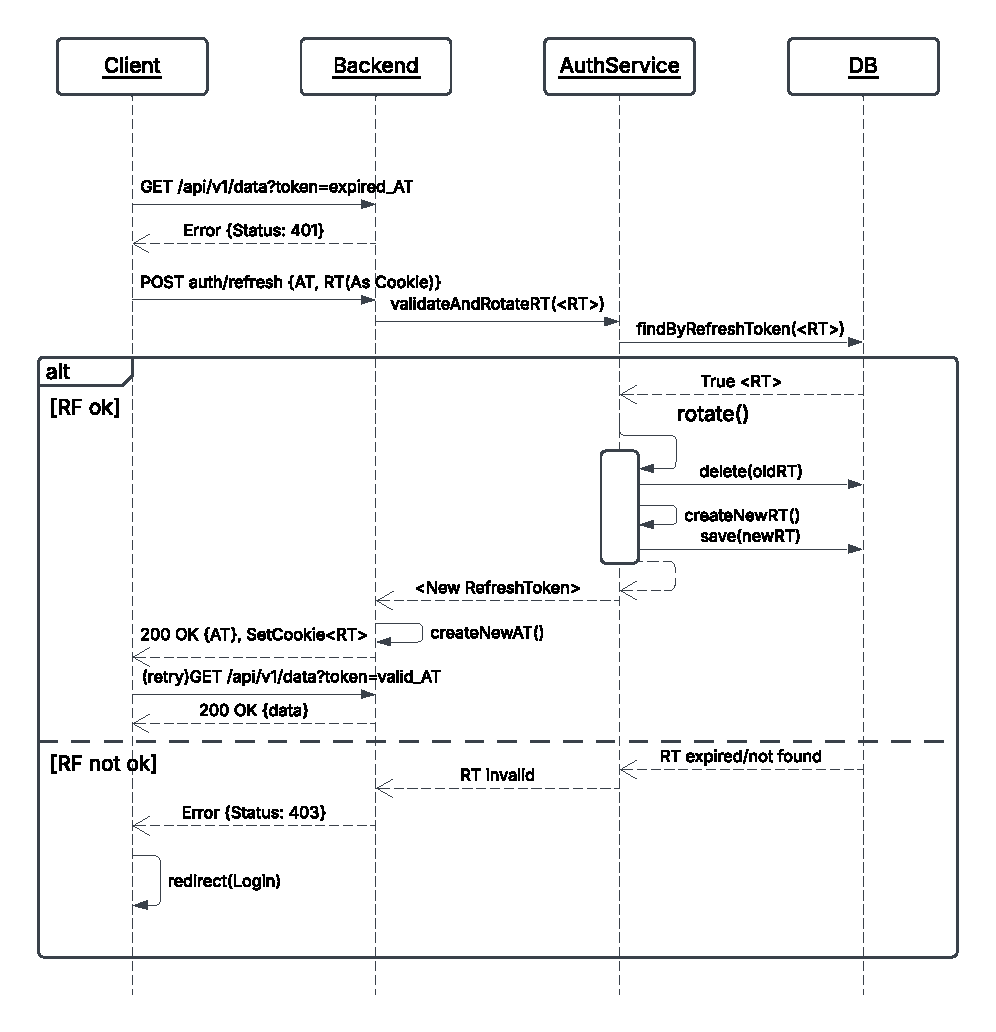
\includegraphics[width=\textwidth]{figures/expired_ac.pdf}
    \caption{Diagramma di sequenza che illustra il flusso di gestione di un Access Token scaduto e la rotazione del Refresh Token, evidenziando le interazioni tra client, backend e database.}
    \label{fig:token_rotation_sequence_uml}
\end{figure}
\vspace{1cm}
%----------------------------------------------------------------------------------------
\chapter{Implementazione}
\label{chap:implementazione}

% Introduzione al capitolo
Questo capitolo illustra i dettagli implementativi salienti del progetto, con l'obiettivo di dimostrare come i concetti e i pattern architetturali discussi nel capitolo di \texttt{Design} (Capitolo \ref{chap:design}) siano stati realizzati concretamente nel codice sorgente. Verranno presentati e analizzati frammenti di codice significativi, sia del backend sviluppato in Java con il framework Spring, sia del frontend in React con TypeScript, evidenziando le scelte tecnologiche e la loro aderenza al disegno progettuale.

\section{Dettagli Implementativi del Backend}
\label{sec:impl_backend}
Il componente backend è stato sviluppato utilizzando Java 17 e il framework Spring Boot 3, con un focus sul paradigma reattivo offerto da Spring WebFlux. Di seguito vengono analizzate le implementazioni dei principali pattern di design adottati.

\subsection{Implementazione del Pattern Factory Method nei Filtri Gateway}
\label{subsec:impl_factory}
% Link di riferimento alla sezione di design
Come descritto nella sezione di design \ref{subsec:design_factory}, il pattern Factory Method è stato utilizzato per creare filtri dinamici nel gateway.

\paragraph{Realizzazione della Factory Concreta}
La classe \texttt{ApiHqAuthGatewayFilterFactory} rappresenta una delle fabbriche concrete. L'annotazione \texttt{@Component} la registra come bean di Spring, rendendola disponibile per l'iniezione delle dipendenze. Il metodo \texttt{apply}, che è l'effettivo "factory method", restituisce una lambda expression che implementa l'interfaccia funzionale \texttt{GatewayFilter}. Questa lambda incapsula la logica per aggiungere l'header di autenticazione \texttt{Basic Auth} a ogni richiesta.

% Includi qui lo snippet di codice Java
% Esempio:
% \begin{lstlisting}[language=Java, caption={Implementazione della factory per il filtro di autenticazione API HQ.}]
% @Component
% public class ApiHqAuthGatewayFilterFactory extends AbstractGatewayFilterFactory<ApiHqAuthGatewayFilterFactory.Config> {
%
%     @Value("${flashstart.apihq.username}")
%     private String apiHqUsername;
%
%     // ... costruttore e altri metodi ...
%
%     @Override
%     public GatewayFilter apply(Config config) {
%         return (exchange, chain) -> {
%             String basicAuthHeader = getBasicAuthHeader();
%             if (basicAuthHeader == null) {
%                 // ... gestione errore ...
%                 return chain.filter(exchange);
%             }
%             ServerHttpRequest request = exchange.getRequest().mutate()
%                     .header(HttpHeaders.AUTHORIZATION, basicAuthHeader)
%                     .build();
%             return chain.filter(exchange.mutate().request(request).build());
%         };
%     }
% }
% \end{lstlisting}

\paragraph{Consumo della Factory nella Configurazione delle Rotte}
La factory viene poi utilizzata in modo dichiarativo nella configurazione delle rotte del gateway, come mostrato in \texttt{GatewayConfig.java}. Il framework invoca il metodo \texttt{apply} al momento opportuno per ottenere l'istanza del filtro da applicare alla rotta specificata.

% Includi qui lo snippet di codice Java della configurazione della rotta

\subsection{Implementazione del Pattern Facade nel Servizio di Autenticazione}
\label{subsec:impl_facade}
% Link di riferimento alla sezione di design
Il pattern Facade, discusso nella sezione \ref{subsec:design_facade}, è stato implementato nella classe \texttt{AuthenticationService} per semplificare il complesso sottosistema di gestione delle sessioni.

\paragraph{Il Metodo \texttt{authenticate}}
Il metodo pubblico \texttt{authenticate} espone un'operazione di business semplice, ma al suo interno orchestra la collaborazione di molteplici componenti: invoca il \texttt{ReactiveAuthenticationManager} di Spring Security per validare le credenziali e, in caso di successo, chiama un metodo privato per generare e salvare il refresh token, nascondendo questa complessità al suo client, l' \texttt{AuthController}.

% Includi qui lo snippet del metodo authenticate() da AuthenticationService.java

\subsection{Implementazione dei Data Transfer Objects (DTO)}
\label{subsec:impl_dto}
% Link di riferimento alla sezione di design
Per realizzare lo scambio di dati disaccoppiato descritto nella sezione \ref{subsec:design_dto}, sono state create delle semplici classi POJO (Plain Old Java Object). Le classi \texttt{AuthRequestDTO.java} e \texttt{AuthResponseDTO.java} definiscono il "contratto" dati per l'API di autenticazione. Il loro utilizzo è evidente nelle firme dei metodi del \texttt{AuthController}, dove vengono usate per mappare il corpo delle richieste e delle risposte HTTP.

% Includi qui gli snippet delle classi DTO e un esempio di firma di un metodo del controller

\section{Dettagli Implementativi del Frontend}
\label{sec:impl_frontend}
Il frontend è stato realizzato con React 18 e TypeScript, sfruttando le funzionalità degli hook per la gestione dello stato e del ciclo di vita dei componenti.

\subsection{Implementazione del Pattern Strategy per i Grafici}
\label{subsec:impl_strategy_frontend}
% Link di riferimento alla sezione di design
Come progettato nella sezione \ref{subsec:design_strategy_frontend}, il pattern Strategy permette di avere un componente \texttt{GenericChart} altamente riutilizzabile.

\paragraph{Definizione delle Strategie}
Le strategie concrete sono definite come oggetti di configurazione nel file \texttt{chartConfigs.ts}. Ogni oggetto implementa l'interfaccia \texttt{ChartConfig}, specificando l'endpoint, la funzione per i parametri e la funzione per la trasformazione dei dati.

% Includi qui lo snippet di un oggetto di configurazione, es. blockedCategoriesConfig

\paragraph{Utilizzo del Componente Contestuale}
La pagina \texttt{Home} istanzia poi molteplici volte il componente \texttt{GenericChart}, passando a ciascuno una diversa strategia tramite la prop \texttt{config}. Questo dimostra come lo stesso componente possa esibire comportamenti radicalmente diversi in base alla strategia iniettata.

% Includi qui lo snippet JSX dalla pagina Home.tsx che mostra l'uso di GenericChart

\subsection{Implementazione del Flusso di Autenticazione Centralizzato}
\label{subsec:impl_auth_frontend}
La gestione centralizzata delle chiamate API e del rinnovo dei token, come da design, è implementata nel file \texttt{axiosInstance.ts}.

\paragraph{L'Intercettore di Risposta}
Il cuore della logica di rinnovo automatico risiede nell'intercettore di risposta. Questo frammento di codice intercetta ogni risposta fallita. Se il codice di stato è \texttt{401}, avvia il processo di refresh, mettendo in attesa le altre richieste e ritentando la chiamata originale al termine del processo.

% Includi qui lo snippet dell'intercettore di risposta da axiosInstance.ts

\paragraph{Gestione dello Stato con React Context}
Il \texttt{AuthContext.tsx} implementa la parte "Observer" del flusso. I metodi \texttt{login} e \texttt{logout} modificano lo stato dell'access token (salvato in memoria tramite \texttt{authStorage.ts}). La modifica di questo stato, condiviso tramite il \textit{provider} del contesto, causa l'aggiornamento automatico di tutti i componenti che usano l'hook \texttt{useAuth()}, come il componente \texttt{PrivateRoute} che decide se renderizzare o meno le pagine protette.

% Includi qui uno snippet da AuthContext.tsx che mostra la funzione di login/logout

\subsection{Implementazione della Sicurezza: Rotazione dei Token}
\label{subsec:impl_security}
% Link di riferimento alla sezione di design
L'implementazione del flusso di rotazione dei token, come descritto nella sezione \ref{sec:design_security_flow}, è il pilastro della sicurezza delle sessioni.

\paragraph{Logica di Rotazione nel Backend}
Il metodo \texttt{validateAndRotateRefreshToken} in \texttt{AuthenticationService.java} è il punto cruciale. Ricevuto un refresh token, esso viene prima cercato nel database. Se trovato e valido, viene immediatamente cancellato per prevenirne il riutilizzo, e solo dopo ne viene generato e salvato uno nuovo, che verrà restituito al client. L'uso dell'annotazione \texttt{@Transactional} garantisce l'atomicità di queste operazioni.

% Includi qui lo snippet del metodo validateAndRotateRefreshToken

\paragraph{Gestione dei Cookie nel Frontend}
Il frontend non interagisce mai direttamente con il refresh token. Il backend lo imposta come cookie \texttt{HttpOnly} tramite l'header \texttt{Set-Cookie}, come visibile nel controller \texttt{AuthController.java}. Il browser si occupa poi di allegare automaticamente questo cookie a ogni richiesta verso il dominio di origine (inclusa la chiamata a \texttt{/auth/refresh}), in modo sicuro e trasparente al codice JavaScript.


\chapter{Metodologia e Infrastruttura di Sviluppo}
\label{chap:metodologia}

% Introduzione al capitolo
Oltre alla progettazione e all'implementazione del software, un progetto di successo si basa su una solida metodologia di sviluppo e su un'infrastruttura di supporto affidabile. Questo capitolo descrive il processo operativo adottato per la realizzazione del progetto, dalla gestione agile alla strategia di testing, fino all'architettura della pipeline di Continuous Integration e Continuous Deployment (CI/CD) che automatizza il rilascio dell'applicazione.

\section{Metodologia di Sviluppo Agile}
\label{sec:metodologia_agile}

Data la natura del progetto come "ponte tecnologico" e i vincoli temporali definiti (RNF5), si è scelto di non adottare un modello a cascata rigido, ma un approccio iterativo e incrementale, ispirato ai principi delle metodologie agili.

\paragraph{Collaborazione con gli Stakeholder} Lo sviluppo è avvenuto in stretta collaborazione con il \textit{product owner} e gli stakeholder aziendali di FlashStart. Questo ha garantito un allineamento costante con le esigenze del business e ha permesso di ricevere feedback tempestivi.

\paragraph{Iterazioni e Demo} Il lavoro è stato organizzato in cicli di sviluppo brevi, assimilabili a degli \textit{sprint}, della durata di circa due settimane. Al termine di ogni ciclo, veniva presentata una demo dello stato di avanzamento del prodotto. Questo approccio ha permesso di:
\begin{itemize}
    \item Validare i requisiti in modo incrementale.
    \item Identificare e correggere eventuali incomprensioni o problemi in una fase precoce.
    \item Mantenere alta la visibilità del progetto all'interno dell'azienda, rafforzando la fiducia degli stakeholder.
\end{itemize}
Questa metodologia si è rivelata vincente per un progetto con requisiti chiari ma che richiedeva flessibilità e velocità di esecuzione.

\section{Strategia di Testing e Validazione}
\label{sec:testing}
Per garantire la qualità, la robustezza e la non regressione del software, è stata implementata una strategia di testing a più livelli, coprendo sia il backend che il frontend.

\subsection{Testing del Backend}
Per il backend Java, sono state implementate due tipologie principali di test, sfruttando il framework di testing JUnit 5 e la libreria Mockito per la creazione di mock.

\paragraph{Unit Test} I test unitari si concentrano sulla verifica del comportamento di singole classi o metodi in isolamento. Un esempio significativo è la classe \texttt{AuthenticationServiceTest}, dove le dipendenze esterne (come \texttt{UserRepository} e \texttt{RefreshTokenRepository}) sono state sostituite con oggetti mock. Questo ha permesso di testare in modo isolato la logica di rotazione dei token, la validazione delle credenziali e la gestione degli errori, senza dipendere da un database reale.

% Potresti inserire un piccolo snippet di un test da AuthenticationServiceTest.java

\paragraph{Integration Test} Per verificare l'interazione tra più componenti, come la logica di servizio e il layer di persistenza, sono stati scritti test di integrazione. Questi test utilizzano un database in-memory H2, configurato per emulare PostgreSQL, come specificato nel file di properties dei test. Ciò permette di testare il flusso completo di salvataggio e recupero dati (es. la creazione di un utente e del suo refresh token) in un ambiente controllato ma realistico.

\subsection{Testing del Frontend}
Per il frontend React, è stata utilizzata la libreria React Testing Library in combinazione con Jest. L'approccio si è concentrato sul testare i componenti dal punto di vista dell'utente.

\paragraph{Component Test} I test verificano che i componenti si renderizzino correttamente e rispondano alle interazioni dell'utente. Un esempio è il test per la pagina di Login, \texttt{Login.test.tsx}, che simula l'inserimento di testo da parte dell'utente, il click sul pulsante di submit e verifica che vengano mostrati i messaggi di errore o di successo appropriati.

\paragraph{Mocking delle Chiamate API} Per isolare i componenti frontend dal backend durante i test, le chiamate API effettuate tramite Axios sono state intercettate e simulate (mocking). Come visibile nei test, l'istanza di \texttt{axiosInstance} viene "mockata" per restituire risposte predefinite, permettendo di testare il comportamento del componente in caso di successo, fallimento o altri scenari di rete.

\section{Deployment e Pipeline di CI/CD}
\label{sec:ci_cd}
Per automatizzare il processo di rilascio e garantire la coerenza degli ambienti, come richiesto da RNF4, è stata progettata e implementata una pipeline di Continuous Integration e Continuous Deployment (CI/CD).

\subsection{Containerizzazione con Docker}
Il fondamento dell'infrastruttura è la containerizzazione. L'intera applicazione (frontend, backend, database) è definita come un insieme di servizi. Questo garantisce che ogni sviluppatore e ogni ambiente di deployment esegua il software con le stesse dipendenze e configurazioni. Sono state utilizzate build multi-stage nei Dockerfile per creare immagini finali ottimizzate e leggere, separando le dipendenze di build da quelle di runtime.

\subsection{Pipeline Ibrida con GitHub Actions e Self-Hosted Runner}
È stata scelta un'architettura di CI/CD ibrida:
\begin{itemize}
    \item \textbf{GitHub Actions} viene utilizzato come orchestratore del flusso di lavoro. La pipeline si attiva automaticamente a ogni push su rami specifici (es. \texttt{main} o \texttt{staging}).
    \item \textbf{Self-Hosted Runner} anziché un runner gestito da GitHub, è stato installato un agente (runner) direttamente sul server di deployment aziendale. Questa scelta strategica garantisce un maggiore controllo e sicurezza: le operazioni di build e deployment avvengono all'interno dell'infrastruttura aziendale, senza esporre credenziali o artefatti all'esterno.
\end{itemize}

\paragraph{Flusso di Deployment} Il flusso tipico della pipeline è il seguente:
\begin{enumerate}
    \item Lo sviluppatore effettua un push sul repository GitHub.
    \item GitHub Actions avvia il workflow definito.
    \item Il job viene assegnato al self-hosted runner.
    \item Il runner esegue i seguenti passi:
          \begin{itemize}
              \item Esegue il build delle immagini Docker per frontend e backend.
              \item Esegue i test automatici per validare la build.
              \item Se i test passano, effettua il push delle nuove immagini su un registry privato (es. Docker Hub).
              \item Esegue il pull delle nuove immagini sul server di deployment.
              \item Riavvia i servizi utilizzando \texttt{docker compose up -d} per applicare l'aggiornamento senza downtime significativo.
          \end{itemize}
\end{enumerate}

% Qui sarebbe perfetto un diagramma che illustra il flusso della pipeline CI/CD
\begin{figure}[h!]
    \centering
    % \includegraphics[width=\textwidth]{path/to/your/ci-cd-pipeline-diagram.png}
    \fbox{Spazio per il diagramma del flusso della pipeline CI/CD}
    \caption{Diagramma che illustra il flusso di Continuous Integration e Continuous Deployment, dal push su Git al deployment sul server.}
    \label{fig:ci_cd_diagram}
\end{figure}

%----------------------------------------------------------------------------------------
% BIBLIOGRAPHY
%----------------------------------------------------------------------------------------

\backmatter

\nocite{*} % Remove this as soon as you have the first citation

\bibliographystyle{alpha}
\bibliography{bibliography}

\begin{acknowledgements} % this is optional
    Optional. Max 1 page.
\end{acknowledgements}

\end{document}
